\documentclass[11pt,a4paper]{article}
\usepackage{fontspec}
\setmainfont{TeX Gyre Pagella}
\newfontfamily\headfont{Inter}[UprightFont=*-ExtraBold,BoldFont=*-ExtraBold,Extension=.otf,Path=/usr/share/fonts/opentype/inter/]
\usepackage[a4paper,margin=2.3cm]{geometry}
\usepackage{graphicx,booktabs,float,caption,array,xcolor,longtable}
\usepackage{xurl}
\usepackage[hidelinks]{hyperref}
\usepackage{titlesec}
\usepackage[round]{natbib}
\usepackage{setspace}
\setstretch{1.05}
\renewcommand{\topfraction}{0.9}
\renewcommand{\bottomfraction}{0.8}
\renewcommand{\textfraction}{0.1}
\renewcommand{\floatpagefraction}{0.75}
\setlength{\parindent}{0pt}
\setlength{\parskip}{0.55em}
\titleformat{\section}{\headfont\Large}{\thesection}{0.8em}{}
\titleformat{\subsection}{\headfont\large}{\thesubsection}{0.8em}{}
\captionsetup{font=small,labelfont=bf}
\urlstyle{same}
\hypersetup{pdftitle={Where Novels Are Set},pdfauthor={Tristan Hotham}}

\begin{document}
\begin{center}
{\Large\bfseries Where Novels Are Set\par}
\vspace{0.4em}
{\large Mapping the real places of fiction in Wikidata:\\7,300 novels, 13,218 literary works and the distance from their authors' birthplaces\par}
\vspace{1.2em}
{\large Tristan Hotham\par}
\vspace{0.3em}
{\small Independent researcher\\
ORCID: 0000-0003-4931-9349\\
DOI: https://doi.org/10.5281/zenodo.23872997\par}
\vspace{0.8em}
2026
\end{center}

\begin{quote}
\small
\begin{center}\textbf{Abstract}\end{center}
I map the narrative locations recorded in Wikidata for every literary work whose setting has coordinates: 13,218 works, of which 7,300 are novels, set in 4,057 distinct real places. Three city areas dominate the novels: London (549 novels), New York (510) and Paris (422), which together appear in 19.9\% of them. Their shares have changed over two centuries: Paris is the setting of 44\% of mapped novels first published from 1830 to 1849, London leads from 1910 to 1949, New York from 1950 to 1989, and London again since 1990. For 6,654 novels with a known author birthplace and setting country, 68.8\% are set entirely within the present-day country of the author's birth; the median distance from birthplace to setting is 343 km and 24.8\% of settings lie within 50 km of it. Europe, with 9.7\% of the world's population, has 53.5\% of the novels; Asia, with 59.5\%, has 9.1\%. Coverage is strongly shaped by contributors: Denmark, with 0.08\% of the world's people, holds 11.7\% of all distinct setting places, more than any other country, and Serbia 3.4\%. The results describe what Wikidata records rather than world literature, and I quantify that difference where I can.

\textbf{Keywords:} literary geography; novels; narrative location; Wikidata; distant reading; digital humanities; open data; mapping
\end{quote}

\section{Introduction}
Literary geography asks where stories happen and why \citep{moretti1998}. Most work in the field studies a single author, city or national literature, because assembling the settings of many books by hand is slow. Wikidata, the collaboratively edited knowledge base behind Wikipedia, now records a narrative location (property P840) for thousands of works, each linked to a place item that usually has coordinates. That makes it possible to draw a world map of fictional settings at the scale of thousands of books, and to ask simple comparative questions. Which cities does fiction favour? How has that changed over time? How far do authors travel from where they were born? Which parts of the world are written about least?

The same data also raise a methodological question. Wikidata is assembled by volunteers, some working through organised projects that add whole national literatures at once. A map of its narrative locations is therefore partly a map of where that effort has gone. I treat this as a finding in its own right and quantify it (Section~\ref{sec:bias}).

\section{Data}
A single query, run with the QLever SPARQL engine \citep{qlever} against Wikidata \citep{wikidata} in 2026, returned every item that is an instance of a subclass of literary work (Q7725634) and has a narrative location whose item has coordinates (P625), with the item's English label, publication date (P577), authors (P50), the coordinates of each author's place of birth (P19), sitelinks and language (P407): 19,443 rows for 13,241 works. Further queries supplied each work's classes (P31), genres (P136), country of origin (P495), languages, form of creative work (P7937), sitelinks and English Wikipedia article, and each place's classes and country (P17). 33 work and place pairs have coordinates on the Moon or Mars; these 23 works set only off Earth are counted but not mapped, leaving 13,218 works with 16,926 settings on Earth in 4,057 places. Country outlines, populations and populated places are from Natural Earth \citep{naturalearth}.

\section{Methods}
\subsection{Novels}
A work is a novel if its form of creative work is novel or novella, or if it is an instance of a class whose English label contains ``novel'' (for example graphic novel or unfinished novel). This gives 7,256 works by form and 56 more by class. I make two exceptions: Wikidata files each of the 67 tales of the Decameron as a ``novella in the Decameron'', and gives the Odyssey's form as novel. Neither is a novel in the usual sense, and both are kept among the literary works only. The result is 7,300 novels. The other 5,918 literary works are mainly plays, short stories, operas and other narratives.

\subsection{Places}
Each place is assigned a level from its Wikidata classes: city or town (1,720 places), site or part of a city such as a street, building or neighbourhood (1,098), wider area such as a state, county, island or region (839), country, former state or civilisation (342), and continent, ocean or world region (58). Places in classes containing ``fictional'' or ``phantom'' (15, such as Arkham or 221B Baker Street) are flagged and excluded from claims about real places. A place's country is the present-day Natural Earth country containing its point (or the nearest within 0.3 degrees); for country-level items the matching Natural Earth country. City areas group every city or site within 25 km of a Natural Earth populated place of at least 250,000 people with that place. ``Set in'' a city, country or continent means that at least one of the work's settings is there.

\subsection{Home and abroad}
An author's home country is the present-day country of their birthplace coordinates. A novel is set at home if all its settings with a country lie in the home country of one of its authors, and abroad otherwise. Distances are great-circle distances from each point setting (city, site or area) to the nearest of the work's authors' birthplaces. Birthplace is not nationality: writers born in colonies, empires or before border changes are assigned to today's country of their birthplace.

\subsection{Genres, periods and fame}
Genres are grouped by regular expressions on Wikidata's genre labels into crime and mystery, science fiction, fantasy, historical fiction, horror and gothic, and children's and young adult fiction. The publication year is the earliest recorded publication date. The number of Wikipedia language editions with an article on a work (sitelinks) is used as a rough measure of fame.

\section{Results}
\subsection{Where novels are set}
Figure~\ref{fig:map} maps the novels' settings. 5,306 novels (72.7\%) have at least one city, site or area; 1,994 name only a country or larger area. Table~\ref{tab:cities} lists the leading city areas. London (549), New York (510) and Paris (422) are far ahead of Los Angeles (140), San Francisco (136), Rome (126) and Madrid (104). Counting all literary works, Paris leads (877). Prolific authors shape the ranking: Pérez Galdós accounts for 37 of Madrid's novels, Rex Stout for 43 of New York's and Simenon for 38 of Paris's. Pittsburgh ranks eighth (98), ahead of Chicago (65); Mumbai has 4 and Lagos 3. By country, the United States has 2,151 novels and the United Kingdom 1,216; together they appear in 45.8\% of all novels.

\begin{figure}[tbp]\centering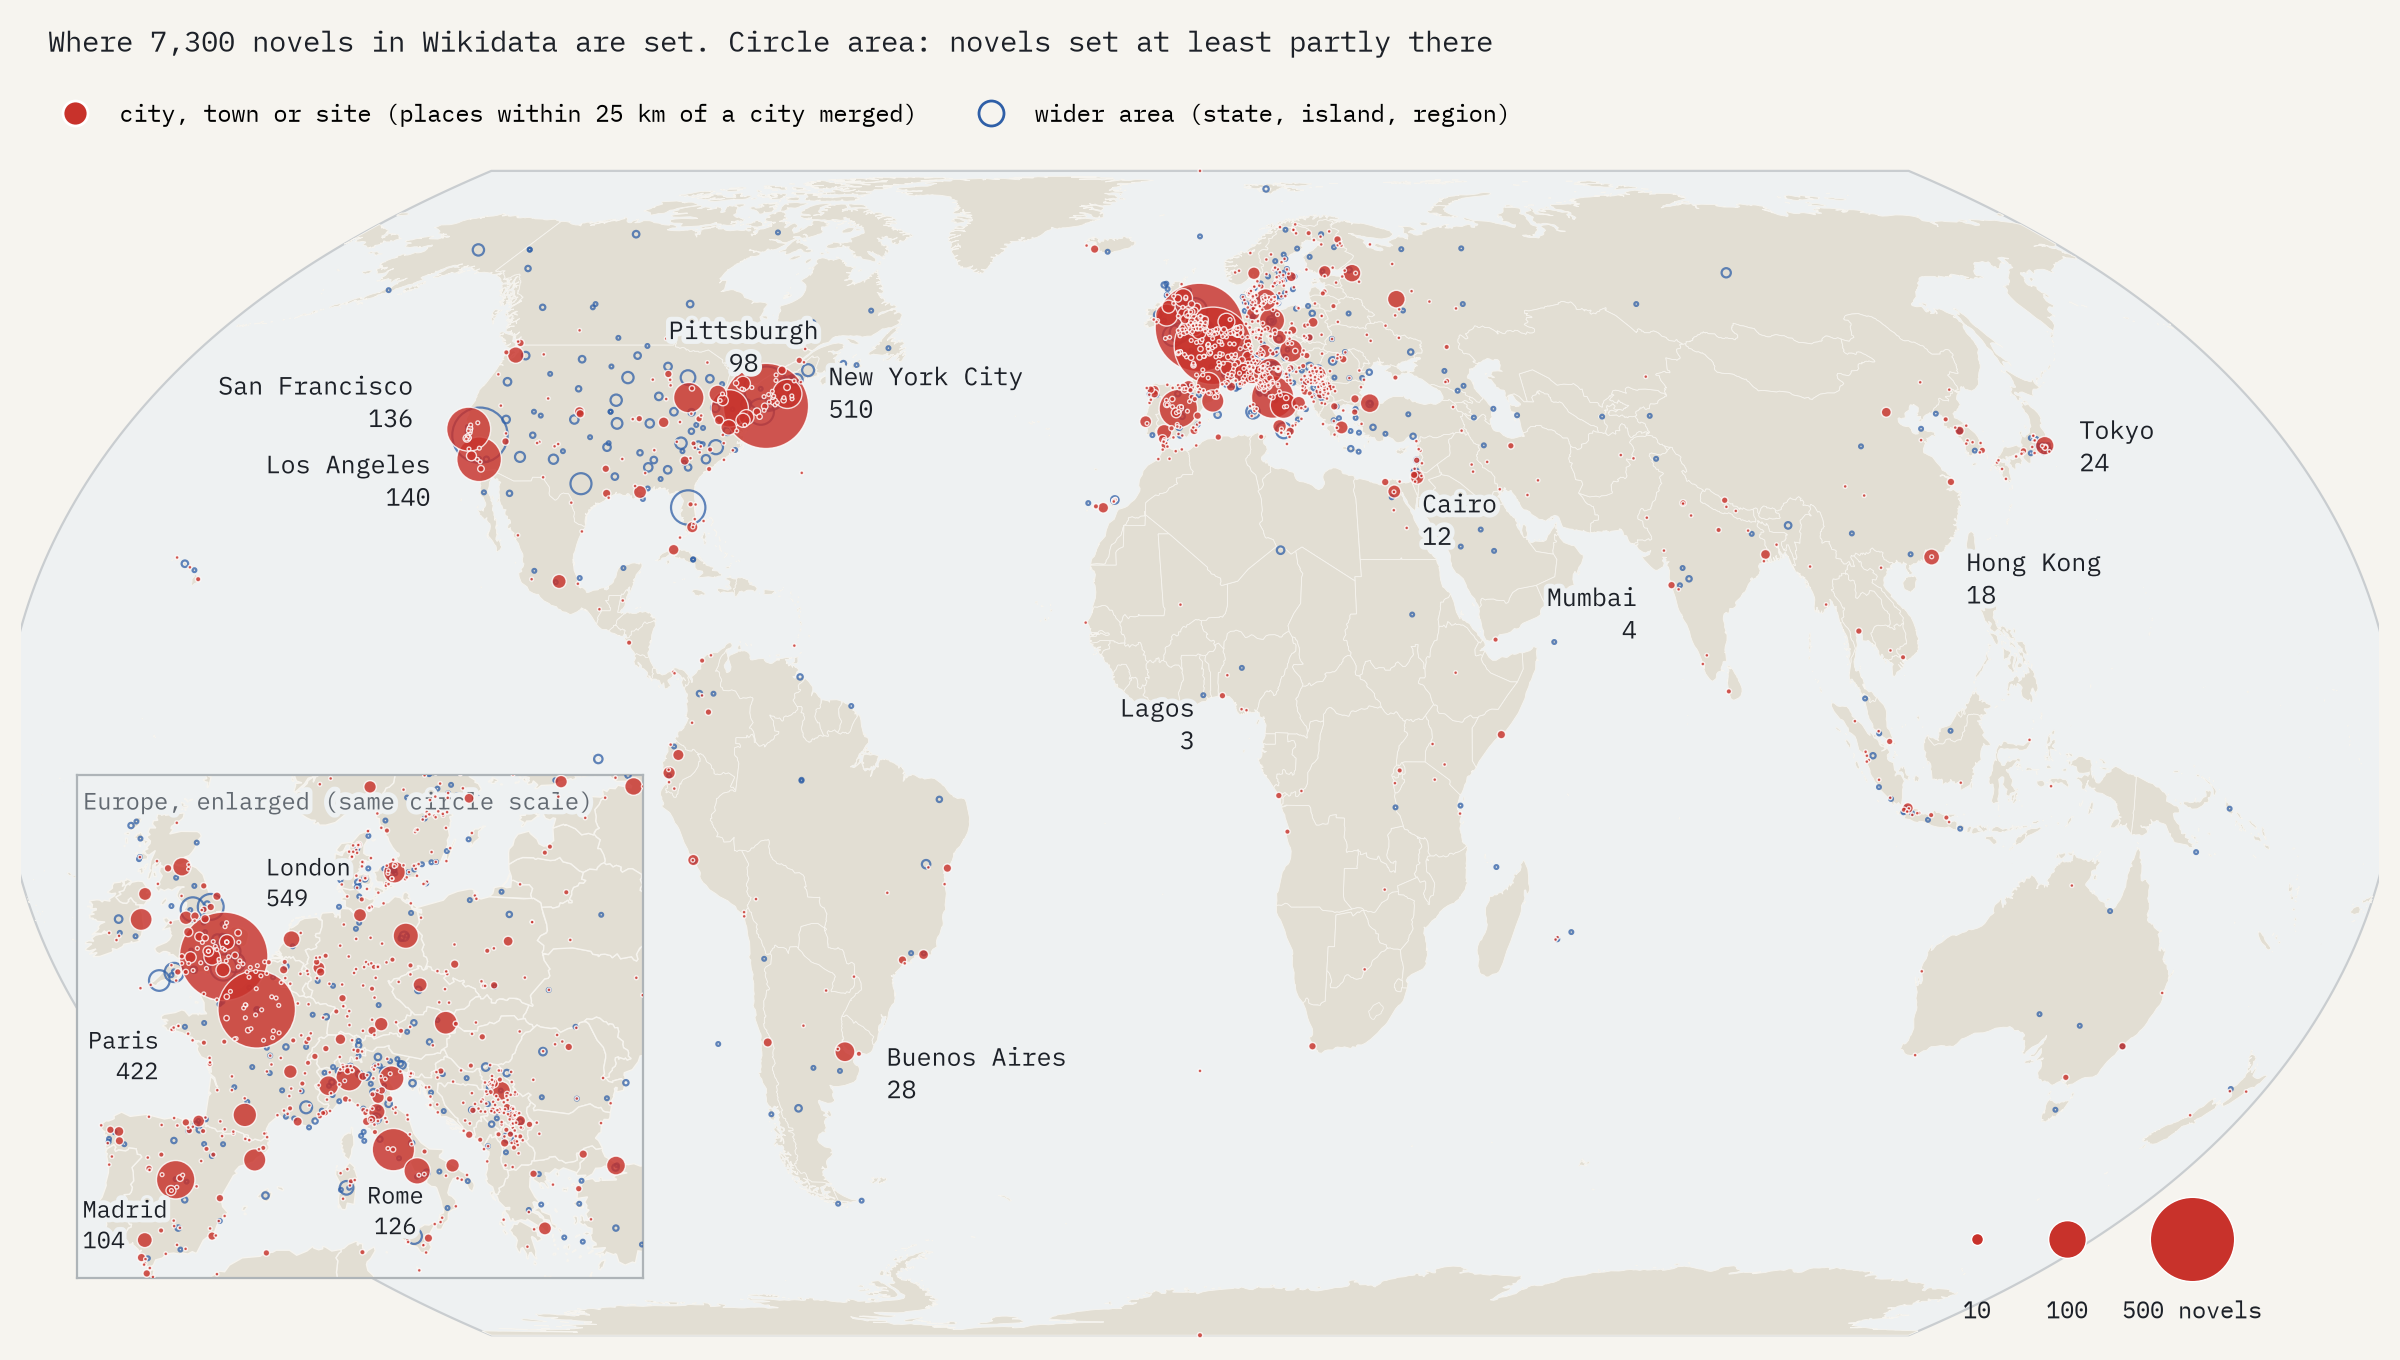
\includegraphics[width=\textwidth]{f_map.png}
\caption{Novels' settings in Wikidata. Filled circles: city areas, towns and sites; rings: wider areas. Circle area is proportional to the number of novels. Inset: Europe at the same circle scale.}\label{fig:map}\end{figure}

\begin{table}[tbp]\centering\small\caption{The twenty city areas with the most novels set at least partly in them, and all literary works.}\label{tab:cities}\begin{tabular}{rllrr}\toprule & City area & Country & Novels & All works\\\midrule
1 & London & United Kingdom & 549 & 786\\
2 & New York City & United States & 510 & 813\\
3 & Paris & France & 422 & 877\\
4 & Los Angeles & United States & 140 & 179\\
5 & San Francisco & United States & 136 & 173\\
6 & Rome & Italy & 126 & 212\\
7 & Madrid & Spain & 104 & 240\\
8 & Pittsburgh & United States & 98 & 103\\
9 & Chicago & United States & 65 & 85\\
10 & Boston & United States & 60 & 80\\
11 & Milan & Italy & 50 & 76\\
12 & Naples & Italy & 49 & 94\\
13 & Berlin & Germany & 45 & 81\\
14 & Venice & Italy & 44 & 81\\
15 & Toulouse & France & 39 & 42\\
16 & Vienna & Austria & 37 & 64\\
17 & Barcelona & Spain & 35 & 41\\
18 & Dublin & Ireland & 34 & 50\\
19 & Copenhagen & Denmark & 33 & 108\\
20 & Turin & Italy & 28 & 29\\
\bottomrule\end{tabular}\end{table}

\subsection{London, Paris and New York over time}
Figure~\ref{fig:trio} shows each city's share of novels with a mapped place by twenty-year period of first publication. Paris is the setting of 44.0\% of novels published from 1830 to 1849 (n = 75), when London has 10.7\% and New York 2.7\%. London and Paris are level from 1890 to 1909, London leads from 1910 to 1949, New York from 1950 to 1989 (15.4\% from 1950 to 1969), and London again since 1990 (11.2\% from 1990 to 2009). Paris falls to 5.0\% from 1990 to 2009. All three shares decline in the most recent period as the settings of recent novels spread over many more places.

\begin{figure}[tbp]\centering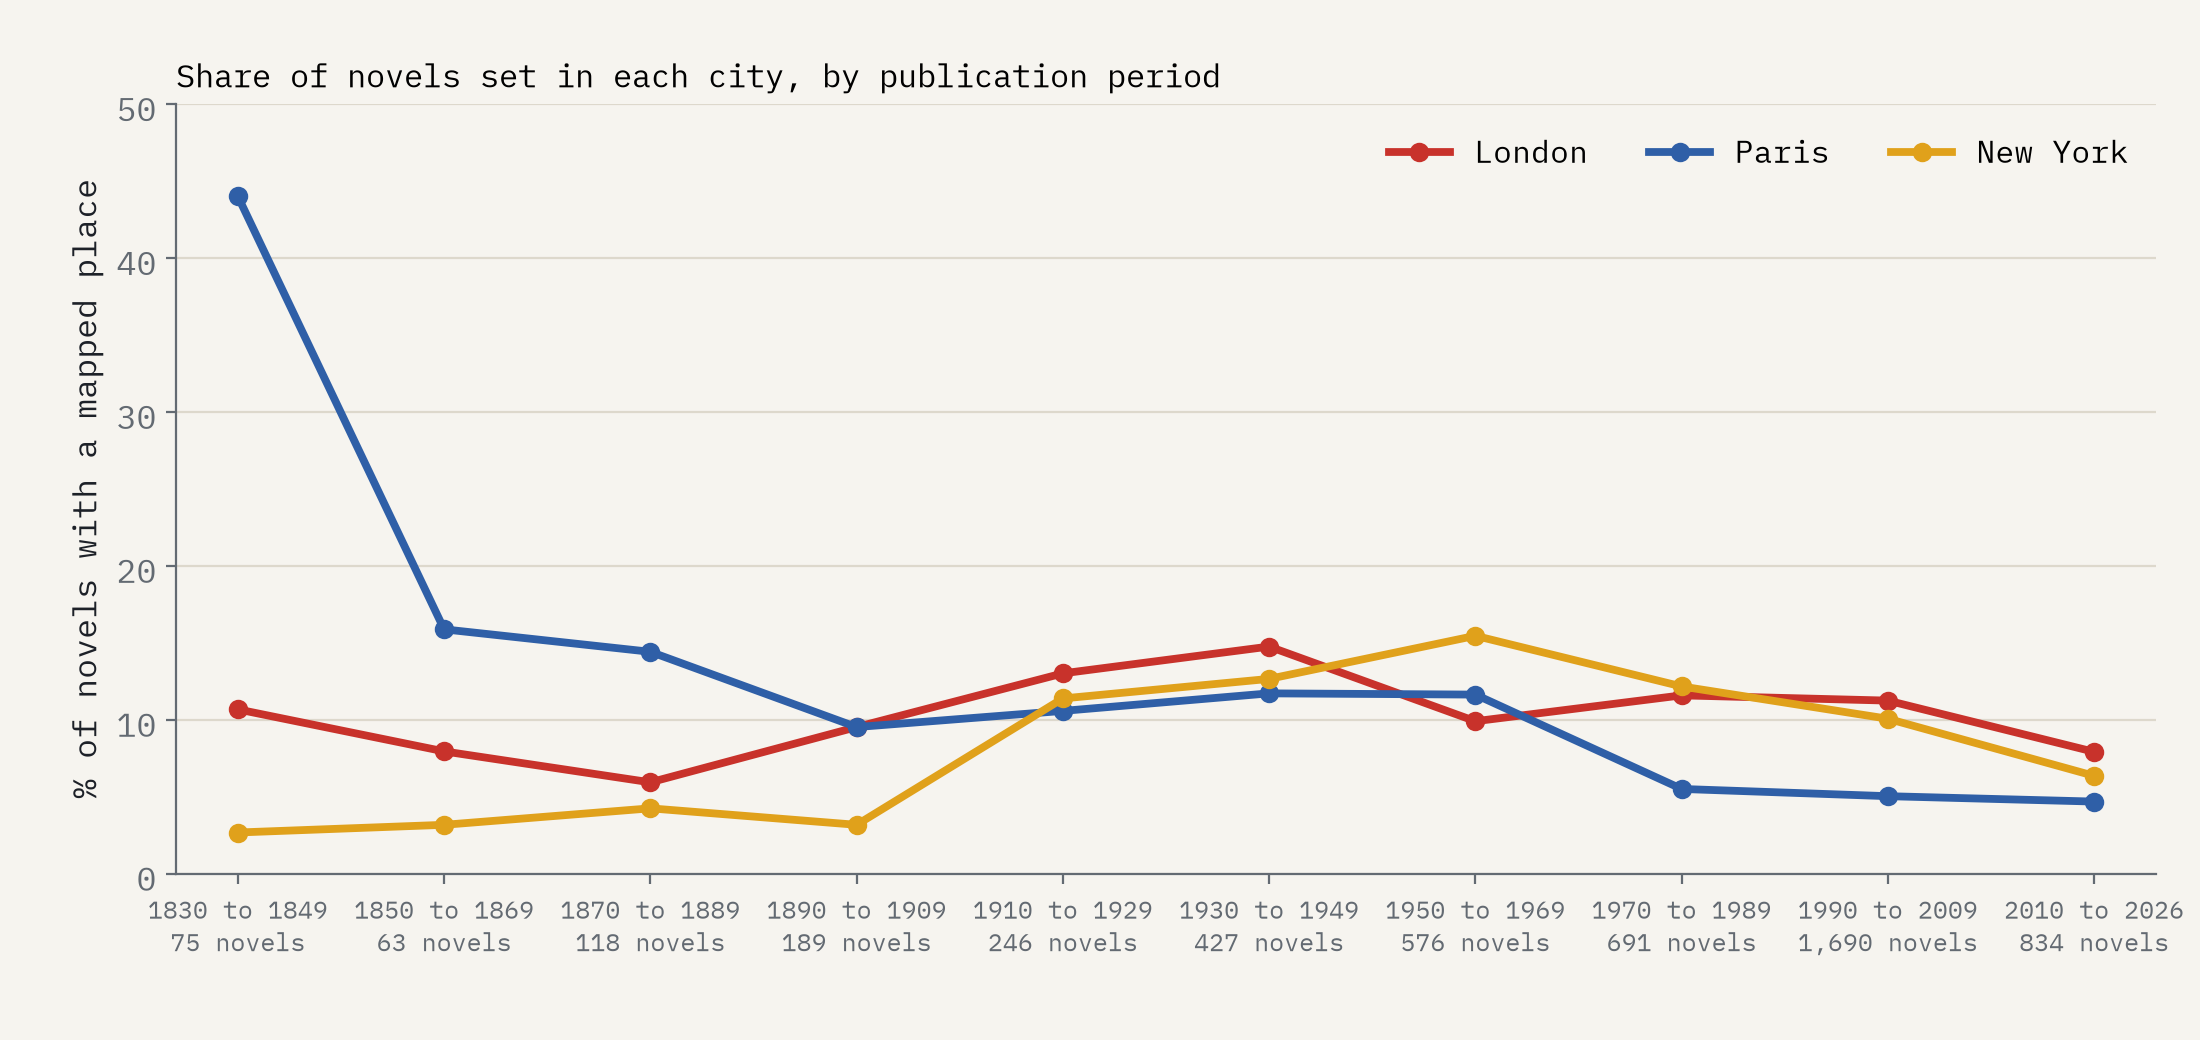
\includegraphics[width=\textwidth]{f_trio.png}
\caption{Share of novels with a mapped place set at least partly in London, Paris and New York, by period of first publication.}\label{fig:trio}\end{figure}

\subsection{Home and abroad}
Of 6,654 novels with a home country and a setting country, 2,079 (31.2\%) are set at least partly abroad and 1,847 (27.8\%) entirely abroad. Across 6,147 novel and point-setting pairs, the median distance from the author's birthplace is 343 km (mean 1,713 km); 24.8\% lie within 50 km, 57.8\% within 500 km and 13.3\% beyond 5,000 km (Figure~\ref{fig:home}). The share abroad ranges by period from 26\% for novels published from 1800 to 1849 to 38\% from 1900 to 1949 and 32\% since 2000. Table~\ref{tab:home} gives the share by birth country. The highest shares reflect the gap between birthplace and nationality: writers born in present-day Ukraine (94\%), Belgium (89\%, chiefly Simenon) and Australia (79\%). American-born writers set 22.3\% of their novels abroad and British-born writers 28.2\%. The longest single journey is Ngaio Marsh's, from Christchurch to Devon in Death at the Bar (19,174 km); among 398 authors with at least three mapped novels, Marsh (median 18,976 km) and P. L. Travers (16,327 km) travel furthest.

\begin{figure}[tbp]\centering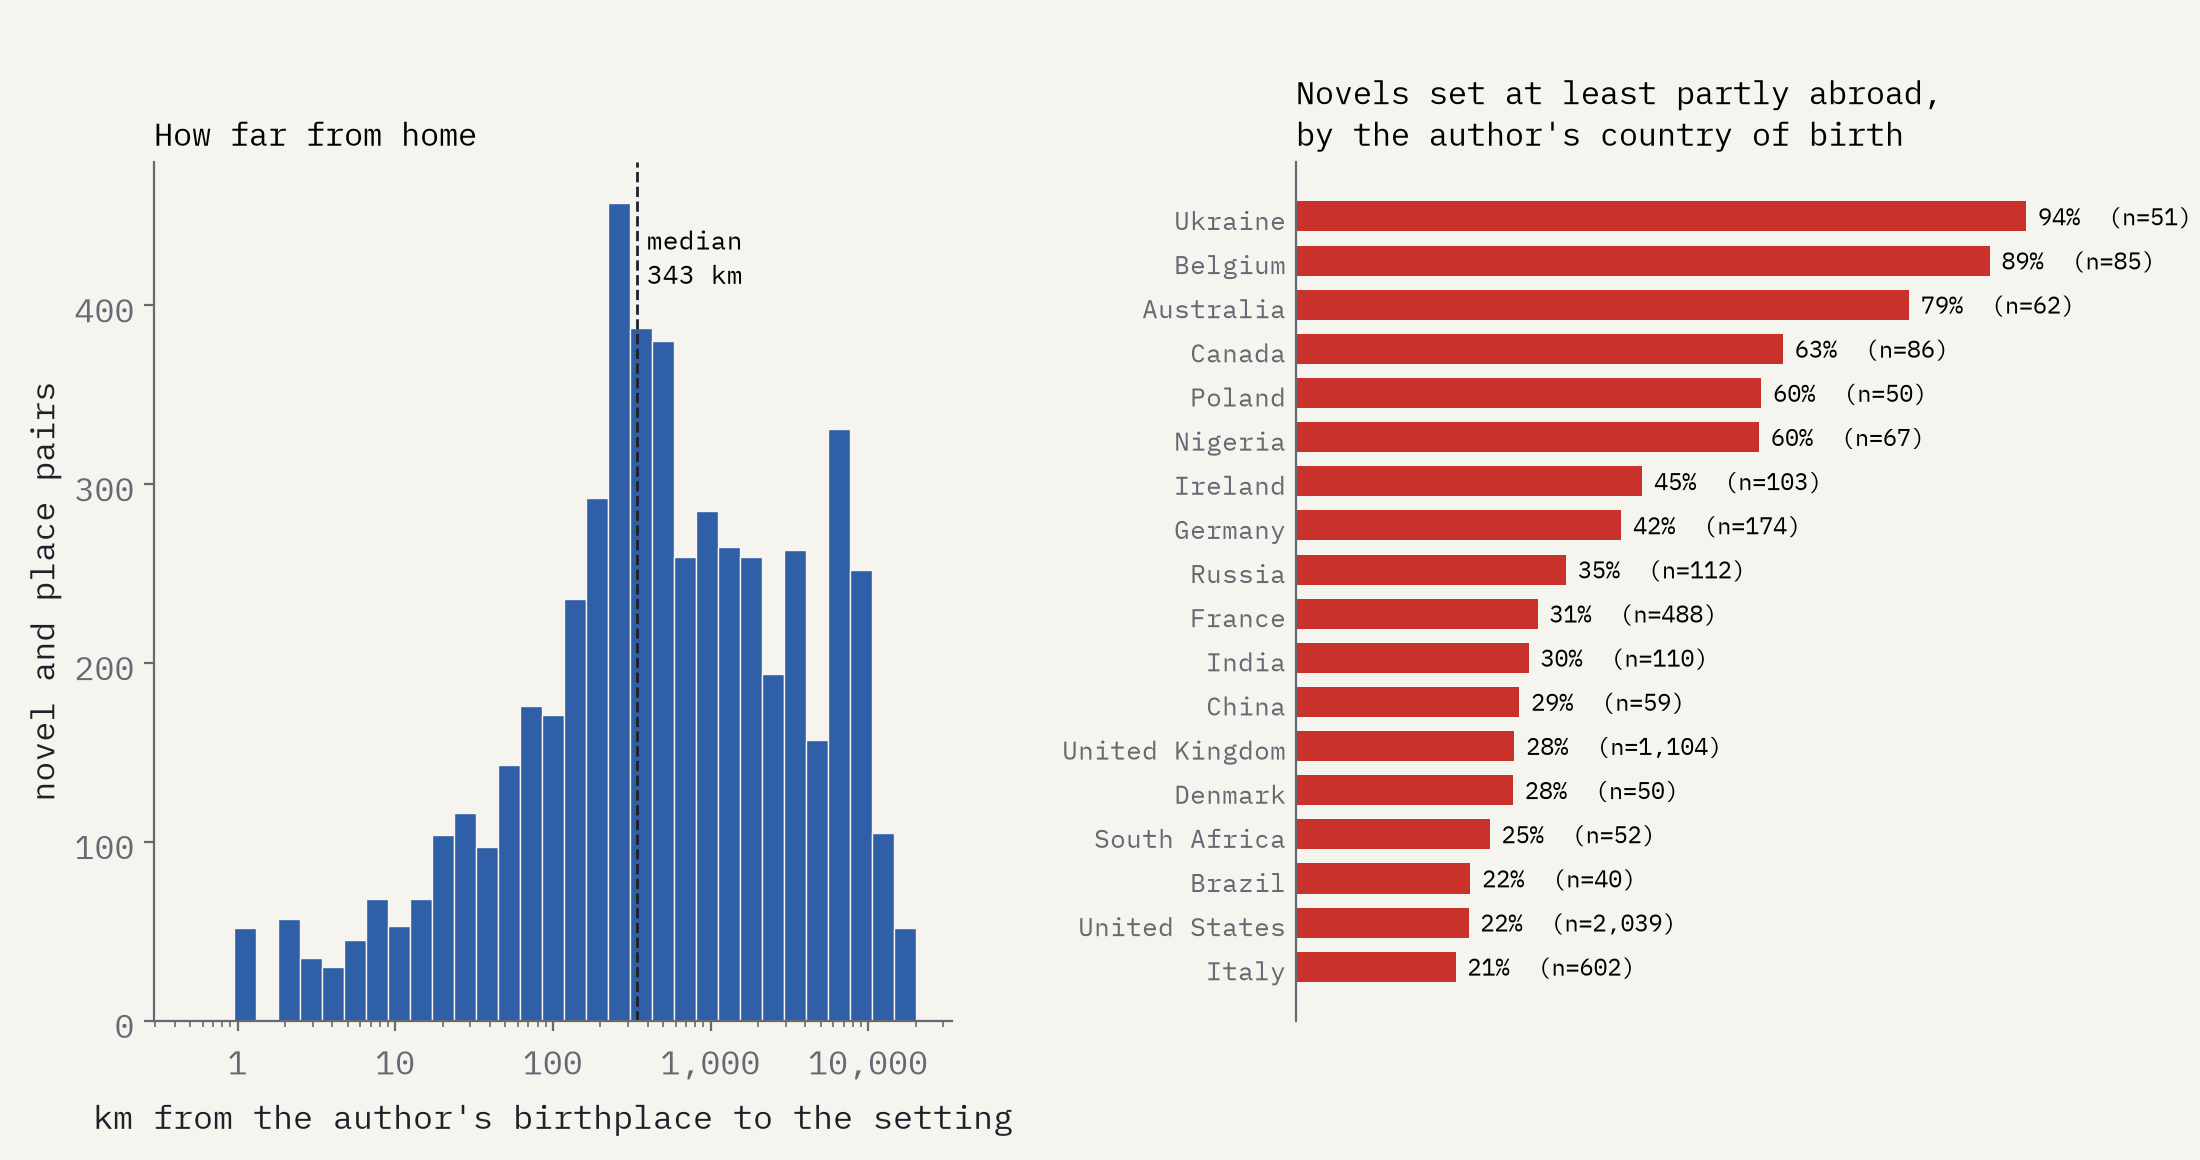
\includegraphics[width=\textwidth]{f_home.png}
\caption{Left: distance from the author's birthplace to each point setting of a novel (log scale). Right: share of novels set at least partly abroad, by present-day country of the author's birthplace (at least 40 novels).}\label{fig:home}\end{figure}

\begin{table}[tbp]\centering\footnotesize\caption{Novels by the present-day country of the author's birthplace (at least 40): share set at least partly abroad, median distance from birthplace to point settings, and the main foreign settings.}\label{tab:home}\begin{tabular}{lrrrp{6cm}}\toprule Born in & Novels & Abroad & Median km & Main foreign settings\\\midrule
Ukraine & 51 & 94.1\% & 1,697 & Russia 11, United States 9, Italy 8\\
Belgium & 85 & 89.4\% & 305 & France 64, United Kingdom 3, China 2\\
Australia & 62 & 79.0\% & 16,327 & United Kingdom 24, Germany 4, Ireland 3\\
Canada & 86 & 62.8\% & 797 & United States 26, United Kingdom 10, China 5\\
Poland & 50 & 60.0\% & 168 & Germany 7, France 4, United States 4\\
Nigeria & 67 & 59.7\% & 5,020 & Italy 24, United Kingdom 6, United States 3\\
Ireland & 103 & 44.7\% & 456 & United Kingdom 25, United States 9, France 5\\
Germany & 174 & 42.0\% & 307 & France 12, United States 11, Italy 10\\
Russia & 112 & 34.8\% & 1,066 & United States 9, Germany 8, France 5\\
France & 488 & 31.1\% & 208 & Egypt 30, Italy 21, United States 21\\
India & 110 & 30.0\% & 5,976 & United Kingdom 14, United States 7, France 3\\
China & 59 & 28.8\% & 8,271 & United Kingdom 6, Canada 3, France 3\\
United Kingdom & 1,104 & 28.2\% & 155 & United States 91, France 39, Ireland 32\\
Denmark & 50 & 28.0\% & 101 & Germany 4, Italy 3, France 2\\
South Africa & 52 & 25.0\% & 8,674 & United Kingdom 5, United States 2, Spain 2\\
Brazil & 40 & 22.5\% & 362 & France 3, United States 2, Egypt 1\\
United States & 2,039 & 22.3\% & 1,020 & United Kingdom 143, France 57, Italy 48\\
Italy & 602 & 20.6\% & 64 & France 16, United States 10, Germany 9\\
Japan & 66 & 16.7\% & 362 & United States 4, China 2, United Kingdom 1\\
Spain & 262 & 16.4\% & 395 & France 15, Italy 7, United States 5\\
Sweden & 91 & 13.2\% & 278 & United States 3, Germany 3, South Africa 1\\
\bottomrule\end{tabular}\end{table}

\subsection{Genres}
Figure~\ref{fig:genres} gives the leading cities for each genre group. Crime and mystery (869 novels) is led by Paris (95), London (82) and New York (59); relative to all novels it is over-represented in Miami, Oslo, Edinburgh and Venice. Science fiction with a real setting (413) goes mostly to New York and London, and is 3.5 times as likely as the average novel to be set in San Francisco; 49.4\% of it is set at least partly in the United States. Fantasy (361) is led by London (47), and historical fiction (586) by Paris, London and New York, with Italy (68 novels) prominent among countries. 25 works are set at least partly on the Moon and 3 on Mars.

\begin{figure}[tbp]\centering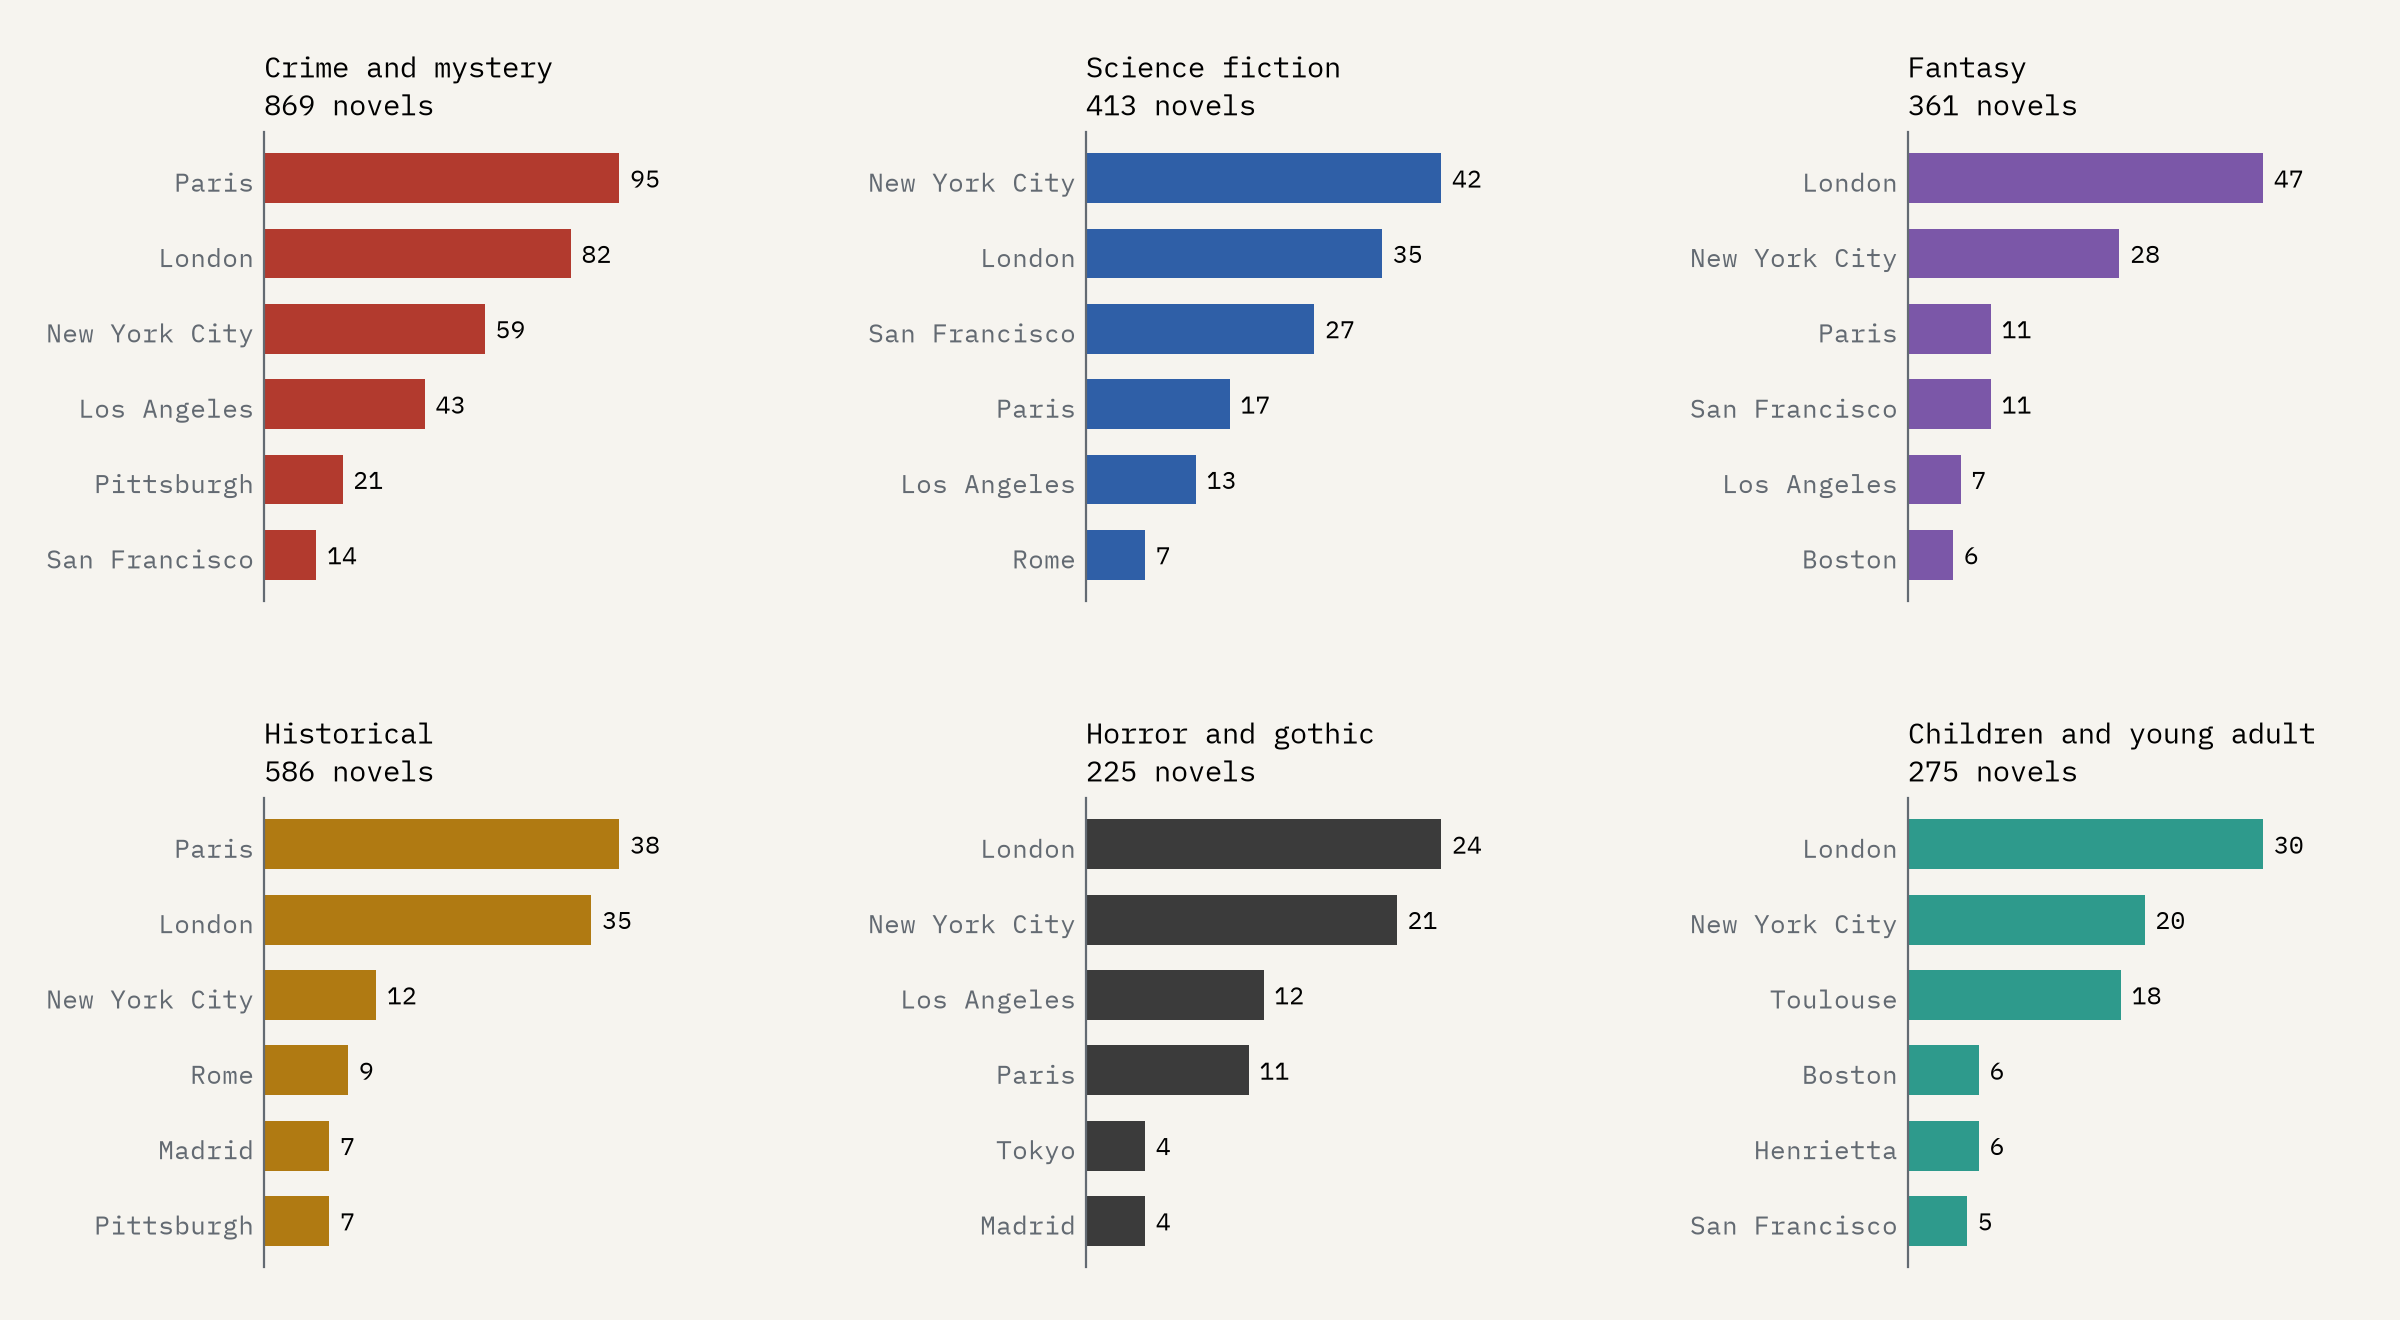
\includegraphics[width=\textwidth]{f_genres.png}
\caption{Leading city areas for each genre group. A novel may belong to more than one group.}\label{fig:genres}\end{figure}

\subsection{Continents and population}
Figure~\ref{fig:conts} and Table~\ref{tab:conts} compare the share of novels set in each continent with its share of world population. Europe has 51.4 novels per 10 million people, North America 39.2, South America 4.2, Africa 2.7 and Asia 1.4. Among countries of 50 million people or more the least mapped are Bangladesh (2 novels), the Philippines (3), the Democratic Republic of the Congo (4), Myanmar (3) and Pakistan (13). 7 countries of more than 10 million people have no mapped novel.

\begin{figure}[tbp]\centering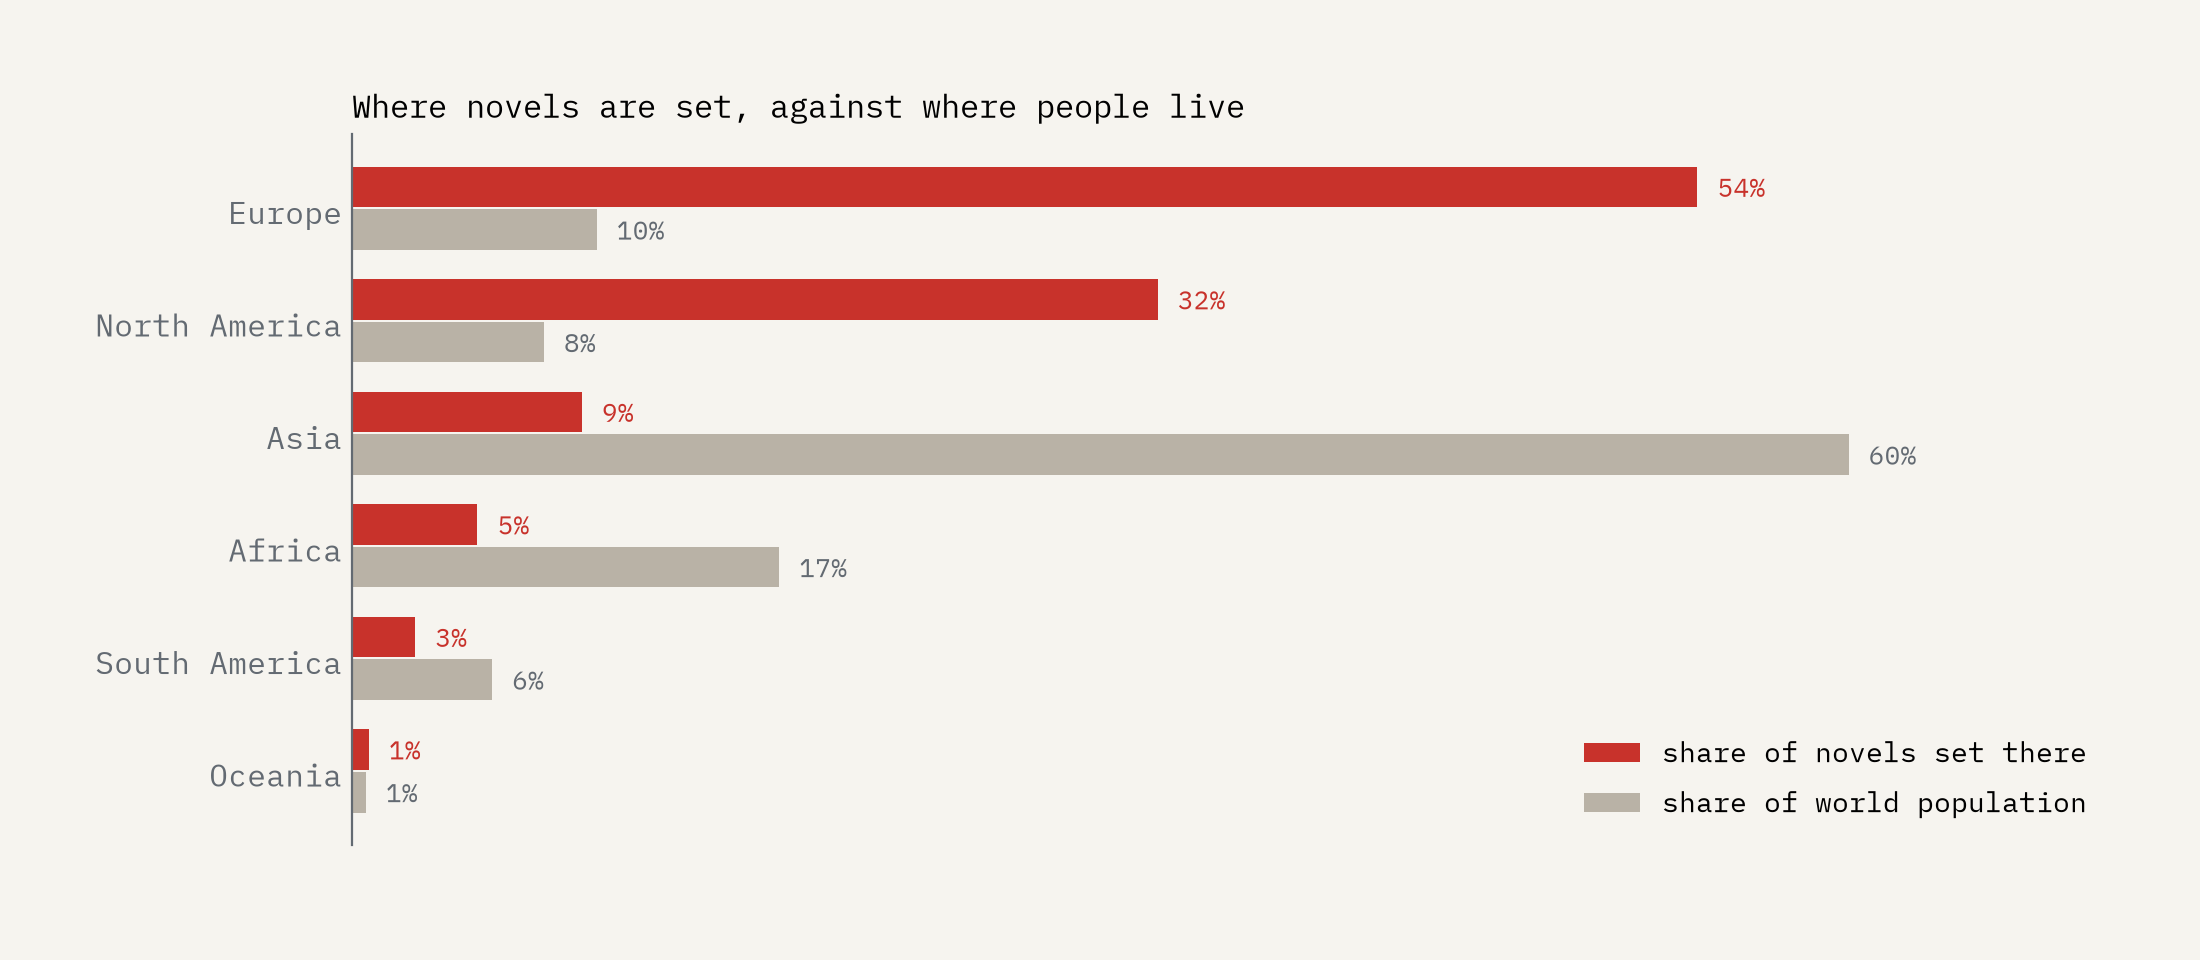
\includegraphics[width=\textwidth]{f_conts.png}
\caption{Share of novels with a setting in each continent (a novel may count for several) against share of world population.}\label{fig:conts}\end{figure}

\begin{table}[tbp]\centering\small\caption{Novels and literary works set at least partly in each continent, share of world population, and novels per 10 million people (not given for Antarctica).}\label{tab:conts}\begin{tabular}{lrrrrr}\toprule Continent & Novels & Share & Works & Population & Per 10m\\\midrule
Europe & 3,836 & 53.5\% & 7,236 & 9.7\% & 51.4\\
North America & 2,297 & 32.0\% & 3,623 & 7.6\% & 39.2\\
Asia & 655 & 9.1\% & 1,440 & 59.5\% & 1.4\\
Africa & 358 & 5.0\% & 621 & 17.0\% & 2.7\\
South America & 180 & 2.5\% & 347 & 5.6\% & 4.2\\
Oceania & 48 & 0.7\% & 107 & 0.6\% & 11.3\\
Antarctica & 7 & 0.1\% & 17 & 0.0\% & n/a\\
\bottomrule\end{tabular}\end{table}

\subsection{Coverage and contributors}\label{sec:bias}
Counting distinct places rather than novels exposes the effect of individual cataloguing efforts (Figure~\ref{fig:bias}). Denmark has 476 distinct setting places (11.7\% of all), more than the United States (410), and 154 times its share of world population; China and India together have 110. Works in Danish average 3.01 settings each against 1.13 for English; one Danish novel, Koordinater, lists 53 places, and 94.8\% of Denmark's places come from works in Danish. 132 of the 189 streets and squares in the data are in Denmark. Serbia has 137 places (37 times its population share), 89.0\% from works in Serbian, which average 5.46 settings and were 95.5\% published before 1930. The novel counts used elsewhere are much less affected: Denmark has 57 mapped novels and Serbia 54. Smaller clusters, such as Pittsburgh's 98 novels and Toulouse's 39, show the same effect at city scale.

\begin{figure}[tbp]\centering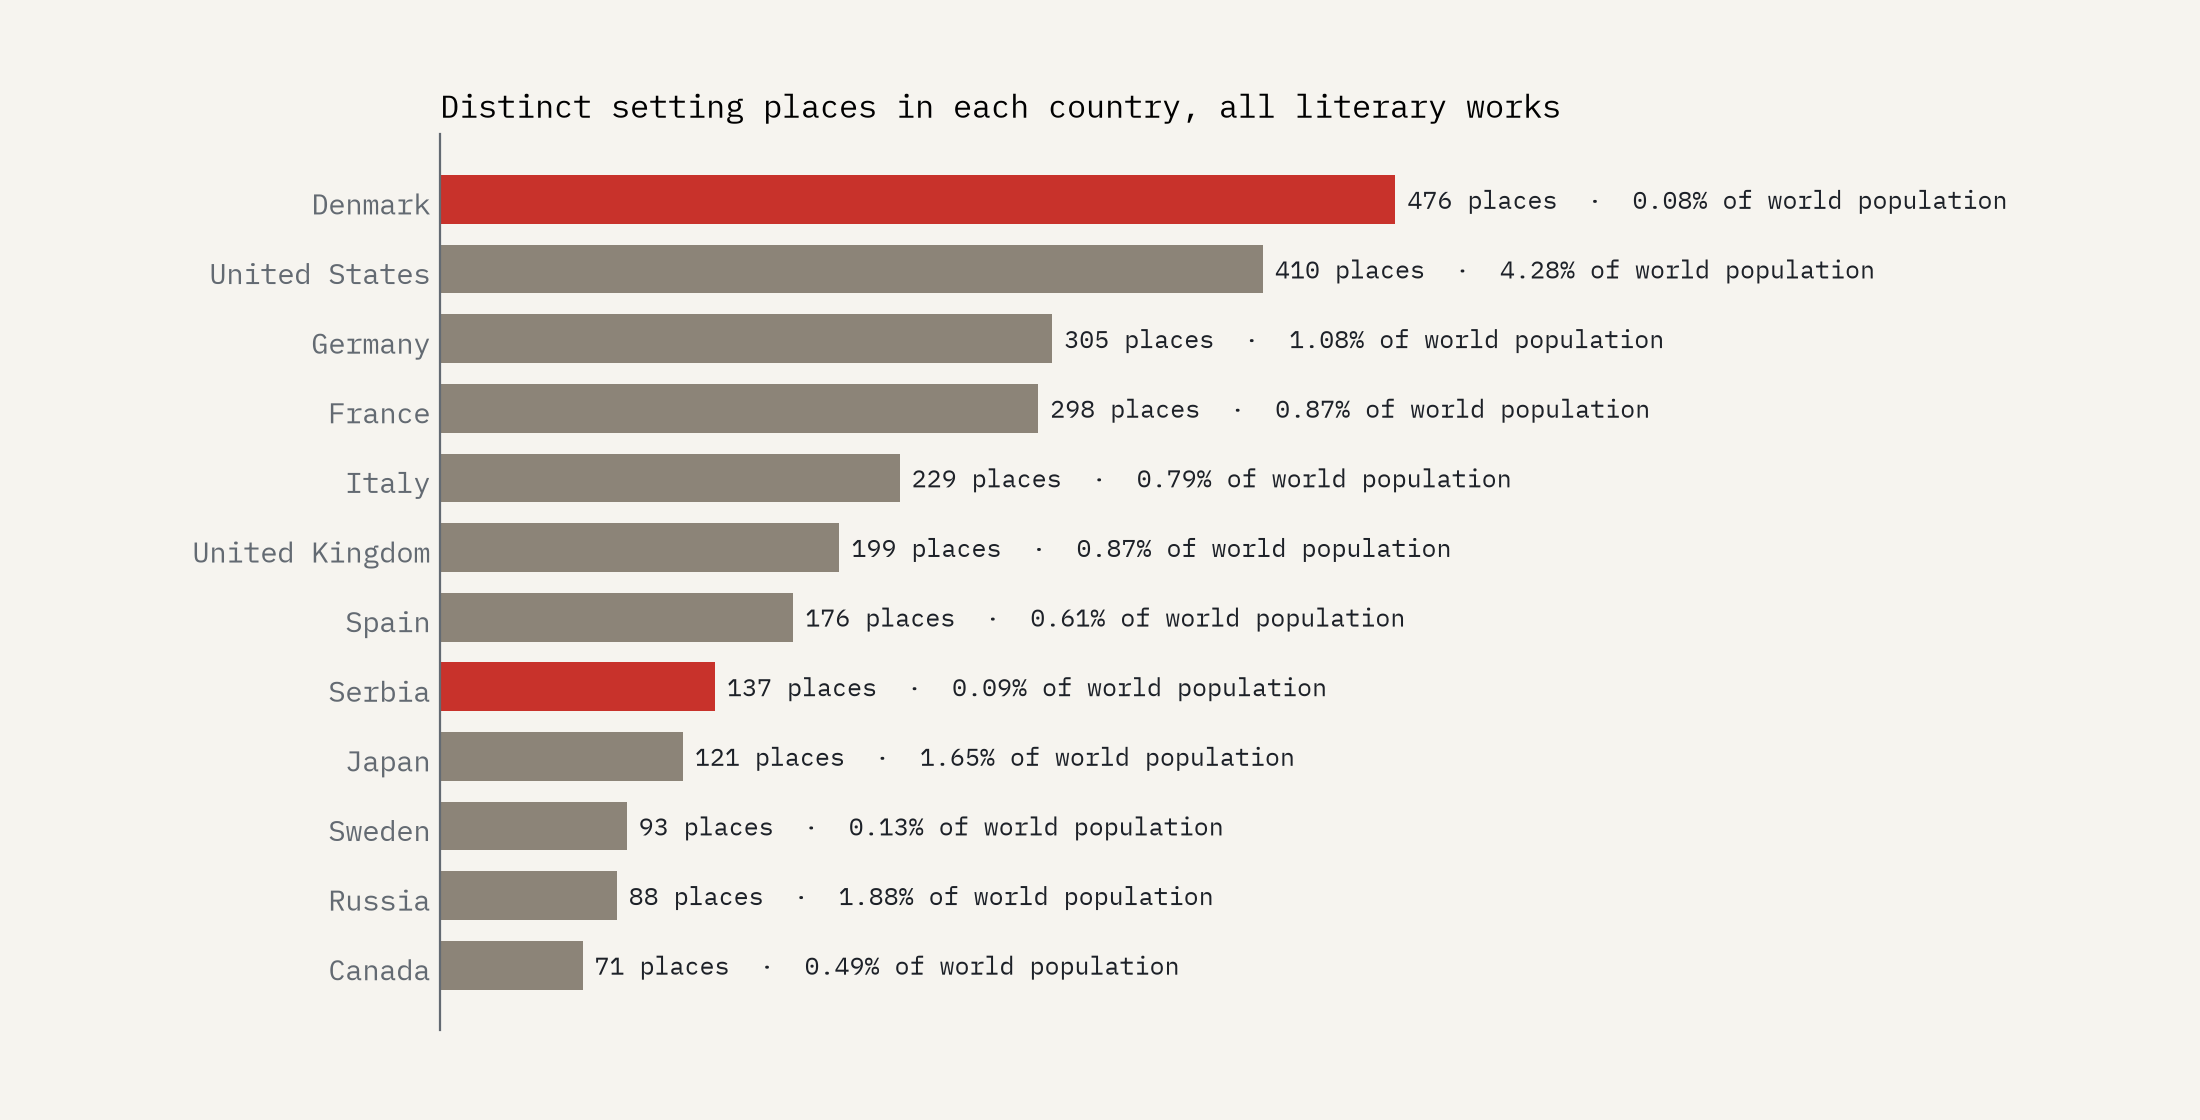
\includegraphics[width=\textwidth]{f_bias.png}
\caption{Distinct setting places by country, all literary works, with each country's share of world population.}\label{fig:bias}\end{figure}

\subsection{Fame and extremes}
The best-known novel in the data by sitelinks is Don Quixote (147 language editions), followed by Nineteen Eighty-Four (138) and Animal Farm (122). Table~\ref{tab:famous} lists the best-known novel set at least partly in each of the leading countries; well-travelled books win in many places (Robinson Crusoe in Venezuela, The Alchemist in Egypt). The most remote real setting, measured as distance to the nearest city of a million people, is the South Pole (5,802 km), followed by islands of French Polynesia (Marquesas Islands, 5,150 km). The northernmost setting is the North Pole. The street with the most works is Istedgade in Copenhagen (4), and the single site is Auschwitz (7).

{\footnotesize\setlength{\tabcolsep}{4pt}\begin{longtable}{lrp{5.2cm}p{3.6cm}rr}\caption{The best-known novel (by Wikipedia language editions) set at least partly in each of the forty countries with the most mapped novels.}\label{tab:famous}\\\toprule Country & Novels & Best-known novel & Author & Year & Links\\\midrule\endfirsthead\toprule Country & Novels & Best-known novel & Author & Year & Links\\\midrule\endhead
United States & 2,151 & The Catcher in the Rye & J. D. Salinger & 1951 & 86\\
United Kingdom & 1,216 & Nineteen Eighty-Four & George Orwell & 1949 & 138\\
Italy & 705 & The Count of Monte Cristo & Alexandre Dumas & 1844 & 79\\
France & 669 & Les Misérables &  & 1862 & 98\\
Spain & 284 & Don Quixote & Miguel de Cervantes & 1605 & 147\\
Germany & 200 & Candide & Voltaire & 1759 & 65\\
India & 158 & Around the World in Eighty Days & Jules Verne & 1872 & 79\\
Russia & 154 & Crime and Punishment & Fyodor Dostoyevsky & 1866 & 109\\
Ireland & 129 & Ulysses & James Joyce & 1922 & 84\\
China & 111 & Dream of the Red Chamber & Cao Xueqin & 1792 & 117\\
Sweden & 91 & The Wonderful Adventures of Nils & Selma Lagerlöf & 1906 & 45\\
Japan & 86 & Around the World in Eighty Days & Jules Verne & 1872 & 79\\
Egypt & 79 & The Alchemist & Paulo Coelho & 1988 & 92\\
Nigeria & 79 & Things Fall Apart & Chinua Achebe & 1958 & 38\\
Canada & 73 & The Call of the Wild & Jack London & 1903 & 54\\
Austria & 69 & War and Peace & Leo Tolstoy & 1869 & 97\\
Denmark & 57 & A Journey to the Centre of the Earth & Jules Verne & 1864 & 64\\
Serbia & 54 & Impure Blood & Borisav Stanković & 1910 & 7\\
Poland & 52 & The Good Soldier Švejk & Jaroslav Hašek & 1921 & 55\\
Mexico & 51 & The Pearl & John Steinbeck & 1947 & 31\\
Turkey & 50 & Candide & Voltaire & 1759 & 65\\
Brazil & 48 & Candide & Voltaire & 1759 & 65\\
South Africa & 47 & Disgrace & J. M. Coetzee & 1999 & 23\\
Argentina & 44 & Candide & Voltaire & 1759 & 65\\
Greece & 41 & Twenty Thousand Leagues Under the Sea & Jules Verne & 1869 & 77\\
Finland & 39 & Colorless Tsukuru Tazaki and His Years of Pilgrimage & Haruki Murakami & 2013 & 28\\
Kenya & 38 & Out of Africa & Karen Blixen & 1937 & 21\\
Netherlands & 37 & The Fault in Our Stars & John Green & 2012 & 50\\
Norway & 37 & Twenty Thousand Leagues Under the Sea & Jules Verne & 1869 & 77\\
Ecuador & 36 & Galápagos & Kurt Vonnegut & 1985 & 17\\
Vietnam & 33 & The Quiet American & Graham Greene & 1955 & 22\\
Australia & 28 & In Search of the Castaways & Jules Verne & 1864 & 47\\
Indonesia & 28 & Max Havelaar & Multatuli & 1940 & 33\\
Czech Republic & 26 & The Good Soldier Švejk & Jaroslav Hašek & 1921 & 55\\
Israel & 26 & The Master and Margarita & Mikhail Bulgakov & 1928 & 79\\
Switzerland & 26 & Angels \& Demons & Dan Brown & 2000 & 63\\
Belgium & 22 & Tintin in the Land of the Soviets & Hergé & 1929 & 29\\
Iran & 22 & Persepolis & Marjane Satrapi &  & 38\\
Portugal & 21 & Candide & Voltaire & 1759 & 65\\
Croatia & 20 & Čuvaj se senjske ruke & August Šenoa & 1876 & 2\\
\bottomrule\end{longtable}}

\section{Limitations}
First, this is a study of Wikidata, not of literature: a work enters only if someone has recorded a narrative location with coordinates, and the records favour books with Wikipedia articles, English labels (2,301 works have none) and active national projects. Second, settings are often partial, and their precision varies from a street to a whole country; some records use a state (New York) where the city is meant. Third, levels, genres and novel status are derived from Wikidata's classes by rules that will misclassify some items. Fourth, home countries use present-day borders and birthplaces, not nationality. Fifth, publication years are the earliest recorded, and recent decades are far better covered than earlier ones (Figure~\ref{fig:decades}).

\begin{figure}[tbp]\centering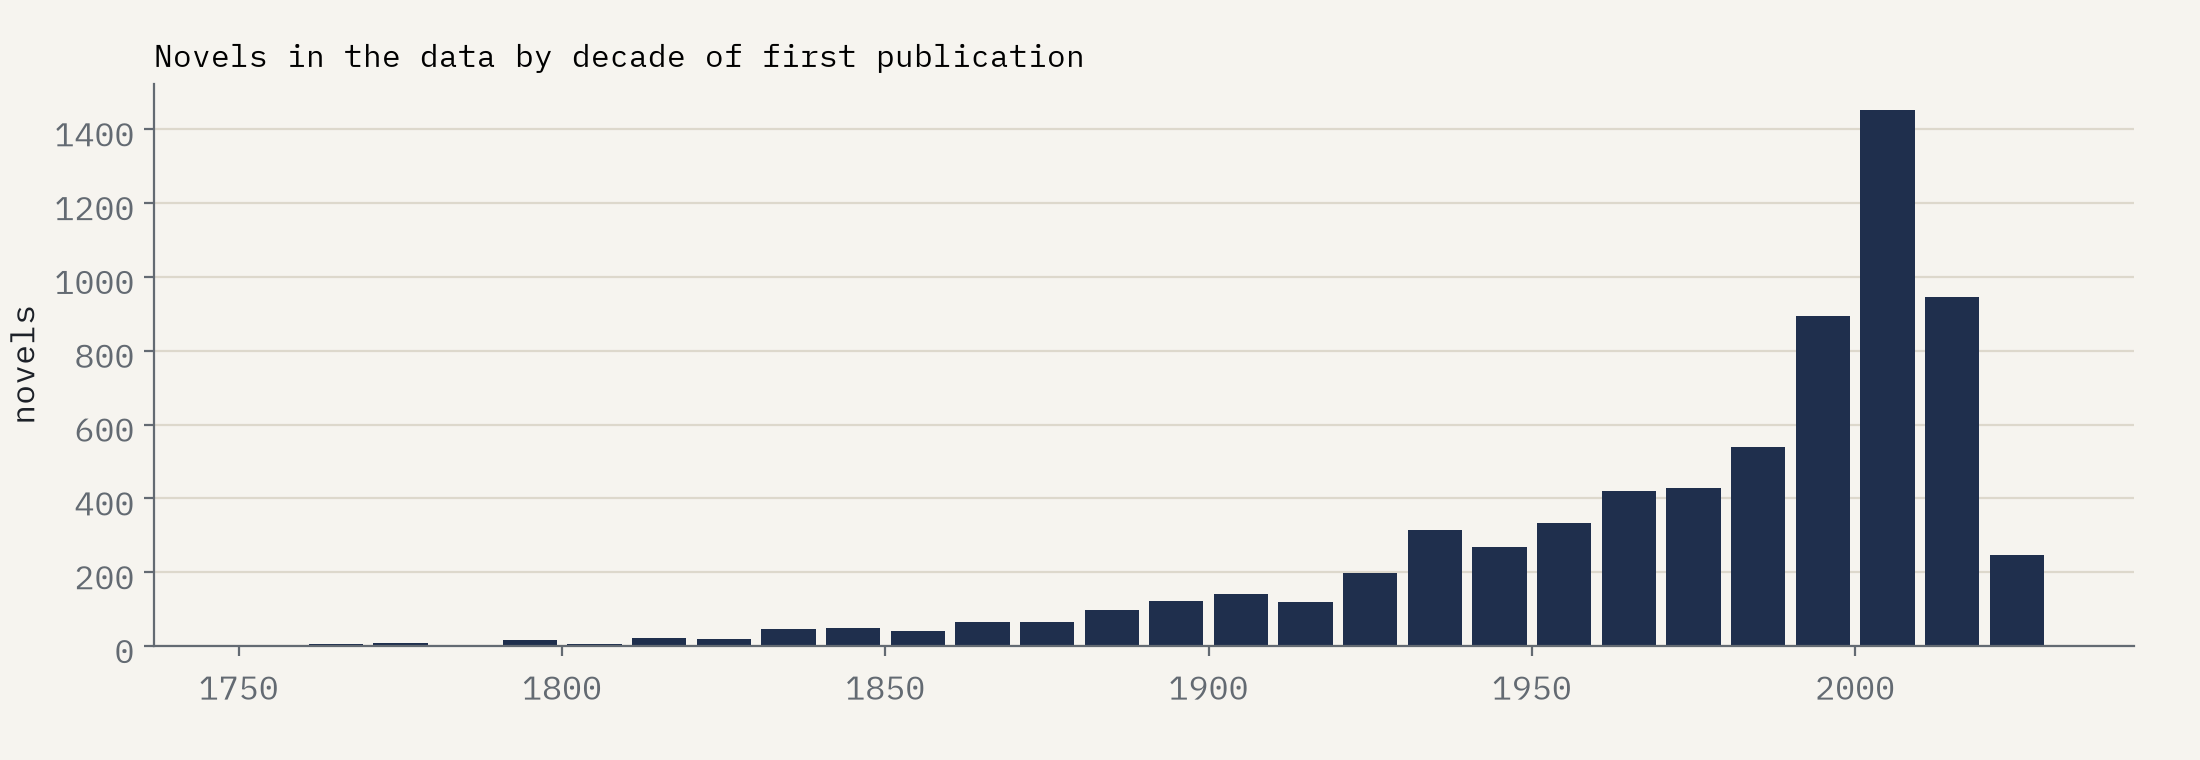
\includegraphics[width=\textwidth]{f_decades.png}
\caption{Novels in the data by decade of first publication.}\label{fig:decades}\end{figure}

\section{Conclusion}
The settings Wikidata records for 7,300 novels describe a fiction that is metropolitan, Euro-American and close to home. Three cities account for about a fifth of the novels, their order has shifted from Paris to London to New York and back to London, and most authors set their stories within a few hundred kilometres of where they were born. The same map shows how strongly open knowledge bases reflect the work of their contributors: a dedicated Danish effort has made Denmark the most finely mapped literary landscape on Earth, while most of Asia and Africa remains thin. Both are worth knowing, and both can change as the data grow.

\section*{Data and code availability}
The interactive map is at \url{https://maps.tristanhotham.com/novel-settings/}. Data and code are at \url{https://github.com/Tristan-Hotham/novel-settings} and archived with this paper at https://doi.org/10.5281/zenodo.23872997. Derived data are released under CC BY 4.0 and code under the MIT licence. Wikidata is CC0.

\section*{AI statement}
I wrote the text, with drafting and editing assistance from Claude (Anthropic), which also helped prepare the analysis code. I reviewed and checked all text and results.

\begin{thebibliography}{9}
\bibitem[Bast and Buchhold(2017)]{qlever} Bast, H. and Buchhold, B. (2017) QLever: a query engine for efficient SPARQL+Text search. Proceedings of CIKM 2017, 647 to 656.
\bibitem[Moretti(1998)]{moretti1998} Moretti, F. (1998) Atlas of the European Novel 1800 to 1900. London: Verso.
\bibitem[Natural Earth(2026)]{naturalearth} Natural Earth (2026) Admin 0 countries and populated places, 1:50m and 1:10m. Public domain. \url{https://www.naturalearthdata.com/}
\bibitem[Vrande\v{c}i\'{c} and Kr\"{o}tzsch(2014)]{wikidata} Vrande\v{c}i\'{c}, D. and Kr\"{o}tzsch, M. (2014) Wikidata: a free collaborative knowledgebase. Communications of the ACM 57(10), 78 to 85. CC0 data at \url{https://www.wikidata.org/}
\end{thebibliography}
\end{document}
